\documentclass[10pt]{beamer}
\usetheme{metropolis}
%\usepackage[utf8]{inputenc}
%\usepackage[T1]{fontenc}
\usepackage{amsmath,amsfonts,amssymb}
\usepackage{mathtools}
\usepackage{relsize}
\usepackage{xspace}
\usepackage{tabu}
\usepackage{comment}
\usepackage{tikz}
\usepackage{epstopdf}
\usepackage{complexity}
\usepackage{framed}
\usepackage{ragged2e}
%\usepackage[usenames, dvipsnames]{color}
%\usepackage{mathpazo}
%\usepackage[beamer,larabove]{tex-local/settings1e}

%\input{tex-local/local_macros}

%\geometry{paperwidth=140mm,paperheight=105mm}
\usepackage{appendixnumberbeamer}

\usepackage{booktabs}
\usepackage[scale=2]{ccicons}

\usepackage{pgfplots}
\usepgfplotslibrary{dateplot}

\usepackage{xspace}
\usepackage{mathtools,amsfonts,amssymb,lmodern}

\usepackage{cryptocode}


\usetikzlibrary[positioning,arrows,scopes,calc,patterns,
backgrounds,decorations.pathmorphing,shapes.geometric]

\title{Rationality and Efficient Verifiable Computation}
\author{Matteo Campanelli}

\date{}

%\institute{The City College of New York\\
%		CUNY}


%\keywords{Rational Proofs, Verifiable Computation}

\AtBeginSubsection[]
{
	\begin{frame}{Outline}
		\tableofcontents[currentsection,currentsubsection]
	\end{frame}
}

%\includeonlyframes{label}

\begin{document}
	
% Theorems

\newenvironment{proofsketch}{\paragraph{\textbf{Proof Sketch:}}}{\hfill$\square$}

\newtheoremstyle{exampstyle}
{5pt} % Space above
{0pt} % Space below
{} % Body font
{} % Indent amount
{\bfseries} % Theorem head font
{.} % Punctuation after theorem head
{.5em} % Space after theorem head
{} % Theorem head spec (can be left empty, meaning `normal')

\theoremstyle{exampstyle}% default 
%\newtheorem{theorem}{Theorem}[section] 
%\newtheorem{lemma}[theorem]{Lemma} 
\newtheorem{proposition}[theorem]{Proposition} 
\newtheorem{property}[theorem]{Property}
%\newtheorem{corollary}[theorem]{Corollary} 

%\theoremstyle{definition} 
%\newtheorem{definition}[theorem]{Definition}
%\newtheorem{conjecture}[theorem]{Conjecture}
%\newtheorem{assumption}[theorem]{Assumption}
%\newtheorem{example}[theorem]{Example}
%\newtheorem{exer}[theorem]{Exercise}

\theoremstyle{plain}
\newtheorem{question}{Question}
\newtheorem{result}{Result}[question]
\newtheorem{resultprogress}{Result (in progress)}[question]

\theoremstyle{definition} 
\newtheorem{remark}{Remark} 





%\def\definition{definition}
%\def\theorem{theorem}
%\def\lemma{lemma}
%\def\corollary{corollary}
%\def\assumption{assumption}
%\def{\remark}{remark}
  
% Tau
\newcommand{\Tau}{\mathcal{T}}

% underbar
%\newcommand{\ubar}[1]{\underaccent{\bar}{#1}}
\newcommand{\ubar}[1]{\uline{#1}}

% Theorems
%\newtheorem{definition}{Definition}
%\newtheorem{lemma}{Lemma}
%\newtheorem{mytheorem}{Theorem}
%\newtheorem{corollary}{Corollary}



% New complexity classes
%\newclass{\DTISP}{DTISP}
\newclass{\NTISP}{NTISP}
%\newclass{\SC}{SC}
\newclass{\NSC}{NSC}
%\newclass{\NC}{NC}
\newclass{\DRMA}{DRMA}
\newclass{\MRIP}{MRIP}

% Rational Proofs
%\newcommand{\A}{Arthur }
%\newcommand{\M}{Merlin }

\newcommand{\Eval}{\mathsf{Eval}}

\newcommand{\nrange}{[n]}

\newcommand{\claimedy}{\tilde{y}}
\newcommand{\posreals}{\reals_{\geq 0}}

\newcommand{\cost}{c}
\newcommand{\disCost}{\tilde{c}}

\newcommand{\costP}{\cost(P,x)}
\newcommand{\xVec}{\widetilde{X}}
\newcommand{\costDisPMany}{m\cdot\costDisP}
\newcommand{\costDisP}{\cost(\disP, x )}

\newcommand{\disP}{\widetilde{P}}
\newcommand{\disPSm}{\widetilde{P}^*}
\newcommand{\bfsP}{\widetilde{P}_{BFS}}

\newcommand{\prCh}{p_{cheat}}
\newcommand{\ratioCosts}{\frac{\cost_H(x)}{\disCLB}}

\newcommand{\function}[1]{\ensuremath{\mathsf{#1}}}

\newcommand{\Size}{\function{Size}}
\newcommand{\out}{\function{out}}
\newcommand{\rew}{\function{rew}}
\newcommand{\profit}{\function{profit}}
%\newcommand{\poly}{\function{poly}}
\def\negl{\function{neg}}
%\newcommand{\reward}{\function{reward}}
%\newcommand{\log}{\function{log}}

\newcommand{\invPoly}{\frac{1}{\poly}}

\newcommand{\expRewProtDis}{\expectation[\rew((\disP,V)(x))]}
\newcommand{\expRewProtDisMany}{\expectation[\rew((\disP,V)(\xVec))]}
\newcommand{\expRewProtHon}{\expectation[\rew((P,V)(x))]}
\newcommand{\prOutProtDis}{\Pr[\out((\disP,V)(x)) \neq f(x)]}
\newcommand{\prOutProtDisMany}{\Pr[\out((\disP,V)(\xVec)) \neq f(\xVec)]}

% expected profit variants
\newcommand{\expProfitProtDis}{\expectation[\profit((\disP,V)(x))]}
\newcommand{\expProfitProtDisMany}{\expectation[\profit((\disP,V)(\xVec))]}
\newcommand{\expProfitProtHon}{\expectation[\profit((P,V)(x))]}

\newcommand{\pDisR}{\tilde{p}_x}

\newcommand{\rnd}{\rho}

\newcommand{\PathCheck}{\function{PathCheck}}

\newcommand{\circuit}{\cal{C}}

\newcommand{\circDFS}{\cal{C}_{DFS}}
\newcommand{\circBFS}{\overline{\cal{C}}_{BFS}}
\newcommand{\circNA}{\overline{\cal{C}}_{NA}}

\newcommand{\circEval}{\cal{C}_{\mbox{eval}}}
\newcommand{\circFFT}{\cal{C}_{\mbox{FFT}}}
\newcommand{\circPow}{\cal{C}_{\mbox{pow}}}

\newcommand{\tildeltaFFT}{\tildelta_{\mbox{FFT}}}

\newcommand{\probCheatFFT}{\tilde{p}_{\mbox{FFT}}}
\newcommand{\probCheatPow}{\tilde{p}_{\mbox{pow}}}

\newcommand{\tildelta}{\tilde{\delta}}
\newcommand{\investTildelta}{\tilde{C}_{\tildelta}}

\newcommand{\deltaBfsInv}{\delta_{BFS}(\tilde{C})}

\newcommand{\disR}{\tilde{R}}
\newcommand{\disRUB}{R'}
\newcommand{\disCLB}{\cost'}

\newcommand{\rewGapOneTime}{\Delta^{\rew}_{1}}
\newcommand{\profGapSeq}{\Delta^{\profit}_{\infty}}
\newcommand{\rewRatio}{\alpha^{\rew}}

% Announced distribution
\newcommand{\annd}{\hat d}
% Real distribution
\newcommand{\reald}{d}

%\newcommand{\expectation}{\mathbb{E}}
\newcommand{\expectation}{\mathop{\mathbb{E}}}

% Some shortcuts for math symbols
\newcommand{\binstrings}{\{0, 1\}^{*}}
\newcommand{\bits}{\{0, 1\}^{*}}
%\newcommand{\iff}{\Leftrightarrow}
\newcommand{\bit}{\{0, 1\}}
\newcommand{\funonstrings}{: \binstrings \to \binstrings}

\newcommand{\naturals}{\mathbb{N}}\label{key}
\newcommand{\reals}{\mathbb{R}}
\newcommand{\field}{\mathbb{F}}

\newcommand{\transp}[1]{{#1}^{\intercal}}


% Circuit Family
\newcommand{\circfam}{\{C_n\}_{n=1}^{\infty}}
\newcommand{\langL}{\mathcal{L}}
% Interactive Proofs
\newcommand{\transc}{\mathcal{T}}

\makeatletter
\newcommand{\verbatimfont}[1]{\def\verbatim@font{#1}}%
\makeatother

\newclass{\BPTISP}{BPTISP}
\newclass{\BPNC}{BPNC}
\newclass{\osDRMA}{osDRMA}
\newclass{\BPRMA}{BPRMA}
%\newclass{\BPQP}{BPQP}
\newclass{\Cclass}{C}

\newcommand{\cb}[1]{\colorbox{BurntOrange}{#1}}
\newcommand{\CN}{\cb{\textbf{[CN]}}}
\newcommand{\XXX}{\cb{\textbf{[XXX]}}}

\begin{comment}
\newtheorem{definition}{Definition}
\newtheorem{lemma}{Lemma}
\newtheorem{claim}{Claim}
\newtheorem{theorem}{Theorem}
\newtheorem{assumption}{Assumption}
\newtheorem{property}{Property}
\newtheorem{question}{Question}
\newtheorem{result}{Result}[question]
\newtheorem{resultprogress}{Result (in progress)}[question]
\newtheorem{corollary}{Corollary}
\end{comment}

\newcommand{\DOM}{\function{DOM}}
\newcommand{\F}{\mathbb{F}}

\newcommand{\allhonest}{\function{all\_honest}}
\def\true{\function{true}}
\def\false{\function{false}}

\newcommand{\Enc}{\function{Enc}}
\def\pk{\function{pk}}
\def\sk{\function{sk}}

 \newcommand{\inprod}[2]{\langle #1 \, , #2 \rangle}


%% Shortcuts specific to Composition
\newcommand{\protOne}{\pi^{f_2}_{1}}
\newcommand{\protTwo}{\pi_{2}}
\newcommand{\rewGap}{\Delta}
\newcommand{\STEP}{STEP}

\newcommand{\disTransc}{\tilde{\Tau}}


\newcommand{\eqdef}{\vcentcolon=}
\newcommand{\binstring}{\{0, 1\}}

\newcommand{\ACzt}{\AC^0[2]}
\newcommand{\ACztq}{\AC^0_{\text{Q}}[2]}
\newcommand{\ACztcm}{\AC^0_{\text{CM}}[2]}

\newcommand{\ACzts}{\AC^0[2]^*}

\def\ANDgt{\function{AND}}
\def\ORgt{\function{OR}}
\def\XORgt{\function{XOR}}


\newcommand{\EqDef}{\stackrel{\mathrm{def}}{=}}

\newcommand{\matr}[1]{\mathbf{#1}}

\newcommand{\unlambda}{1^{\lambda}}
\newcommand{\lambdabits}{\bit^{\lambda}}
\newcommand{\GF}{\text{GF}}
 

\newcommand{\ens}[1]{\{#1_{\lambda}\}_{\lambda\in\naturals}}
\newcommand{\funfam}[1]{\{#1_{\lambda}\}_{\lambda\in\naturals}}

\def\lind{\sim_{\Lambda}}


% == BEGIN Public-Key Encryption ==
\newcommand{\PKE}{\function{PKE}}
\newcommand{\PKEKeygen}{\function{PKE.Keygen}}
\newcommand{\PKEEnc}{\function{PKE.Enc}}
\newcommand{\PKEDec}{\function{PKE.Dec}}
% == END Public-key Encryption ==

% == BEGIN DVV16 ==
\def\M{\matr{M}}
\def\Mz{\matr{\hat{M}}_0^{\lambda}}
\def\Mo{\matr{\hat{M}}_1^{\lambda}}

\newcommand{\KSample}{\function{KSample}}

\def\r{\mathbf{r}}
\def\k{\mathbf{k}}
\def\c{\mathbf{c}}
\def\t{\mathbf{t}}

% == END DVV16 ==

% == BEGIN Homomorphic Encryption ==
\providecommand{\evk}{\pckeystyle{evk}}


\newcommand{\HE}{\function{HE}}
\newcommand{\HEKeygen}{\function{HE.Keygen}}
\newcommand{\HEEnc}{\function{HE.Enc}}
\newcommand{\HEDec}{\function{HE.Dec}}
\newcommand{\HEEval}{\function{HE.Eval}}

\newcommand{\HEp}{\function{HE'}}
\newcommand{\HEpKeygen}{\function{HE'.Keygen}}
\newcommand{\HEpEnc}{\function{HE'.Enc}}
\newcommand{\HEpDec}{\function{HE'.Dec}}
\newcommand{\HEpEval}{\function{HE'.Eval}}

\def\A{\mathbf{A}}
\def\v{\vect{v}}
\def\a{\vect{a}}
\def\Sum{\mathlarger{\sum}}
\def\kl{\k_{\ell}}
\def\klp{\k_{\ell+1}}


\def\Dl{\mathcal{D}^{\func{f}}_{\lambda}}
\def\MD{\M^{\mathcal{\func{f}}}}
\def\Mkg{\M^{\text{kg}}}

% == END Homomorphic Encryption ==

% == BEGIN proof security HE (crypto 2018) ==
\def\hE{\mathcal{E}}
\def\hEz{\hE^{0}}
\def\hH{\mathcal{H}}
\def\hHz{\hH^{0}}

\def\valpha{\pmb{\alpha}}
\def\valphakg{\valpha^{\func{kg}}}
\def\valphaD{\valpha^{\func{f}}}
\def\hEnc{\function{E}}
% == END proof security HE (crypto 2018) ==

% == BEGIN Delegation of Computation ==
\newcommand{\Del}{\function{Del}}
\def\D{\function{D}}
\def\W{\function{W}}
\newcommand{\DW}{\langle \D, \W \rangle}

\def\skD{\sk_{\D}}
\def\pkW{\pk_{\W}}

\newcommand{\advstar}{\adv^*}

 
\newcommand{\hatr}{\hat{r}}
\newcommand{\hatw}{\hat{w}}
\newcommand{\hatF}{\hat{f}}

\def\zero{\bar{0}}
\def\raux{\vect{r}_{\text{aux}}}
\newcommand{\hatraux}{\vect{\hat{r}}_{\text{aux}}}

\newcommand{\hatzpi}[1]{\hat{z}_{\pi(#1)}}

\def\Gvc{{\cal G}}
\def\Wstar{\W^*}

\def\hatx{\hat{x}}
\newcommand{\hatq}{\hat{q}}
\newcommand{\hata}{\hat{a}}
\def\hats{\hat{s}}
\def\Doffline{\D_{\text{off}}}
\def\Donline{\D_{\text{on}}}
\newcommand{\Dverif}{\D_{\text{ver}}}

\newcommand{\VCKG}{\function{VC.KeyGen}}
\newcommand{\VCPG}{\function{VC.ProbGen}}
\newcommand{\VCCompute}{\function{VC.Compute}}
\newcommand{\VCVerif}{\function{VC.Verify}}

\newcommand{\tVCKG}{\function{\overline{VC.KeyGen}}}
\newcommand{\tVCPG}{\function{\overline{VC.ProbGen}}}
\newcommand{\tVCCompute}{\function{\overline{VC.Compute}}}
\newcommand{\tVCVerif}{\function{\overline{VC.Verify}}}

\newcommand{\qx}{q_x}
\newcommand{\sx}{s_x}
\newcommand{\ax}{a_x}

\def\fail{\bot}

\def\VC{{\cal VC}}
\def\tVC{\overline{{\cal VC}}}


\newcommand{\expVC}[1]{{\bf Exp}^{\function{Verif}}_{A}[#1, f, \lambda, l,m]}
\newcommand{\expVCone}[1]{{\bf Exp}^{\function{Verif}}_{A}[#1, f, \lambda, 1,1]}
\newcommand{\expVCmany}[1]{{\bf Exp}^{\function{Verif}}_{A}[#1, f, \lambda, O(1), \poly(\lambda)]}


\newcommand{\hatzpip}[1]{\hat{z}_{\pi'(#1)}}
\newcommand\given[1][]{\:#1\vert\:}


\newcommand{\tpkW}{\pkW}
\newcommand{\tskD}{\skD}
\newcommand{\tqx}{\overline{\qx}}
\newcommand{\tsx}{\overline{\sx}}
\newcommand{\tax}{\overline{\ax}}


% == END Delegation of Computation==

\def\ANDgt{\function{AND}}
\def\ORgt{\function{OR}}
\def\XORgt{\function{XOR}}


\newcommand{\pLpoly}{\oplus \L / \poly}
\newcommand{\fgAssump}{\NC^1 \subsetneq \pLpoly}
	

\frame[plain,label=title]{\titlepage}



\begin{frame}[allowframebreaks]
	\frametitle{References}
	\bibliographystyle{amsalpha}
	\bibliography{references.bib}
\end{frame}



\section{Introduction}

\begin{frame}{Motivation}

\end{frame}


% Metaphor
\begin{frame}{My Thesis, Succinctly}
	
\end{frame}

% Papers
\begin{frame}{Related Papers}
	
\end{frame}



%
\section{Background on Rational Proofs}
\begin{frame}{Overview of Rational Proofs [AM12]}
\begin{itemize}[<+- | alert@+>]
	\item A variant of interactive proofs where the verifier pays the prover at the end;
	\item \textbf{Soundness:}
	\begin{itemize}
		\item ``A cheating worker gains less than an honest one''
	\end{itemize}
%	\item Other desiderata:
%	\begin{itemize}
%		\item Reward should be higher than cost (\textit{individually rational})
%		\item Ensuring ``significant'' losses for cheaters;
%		\item Ensuring ``compact'' budget for delegators.
%	\end{itemize}
\end{itemize}
\onslide<1->
\begin{figure}
	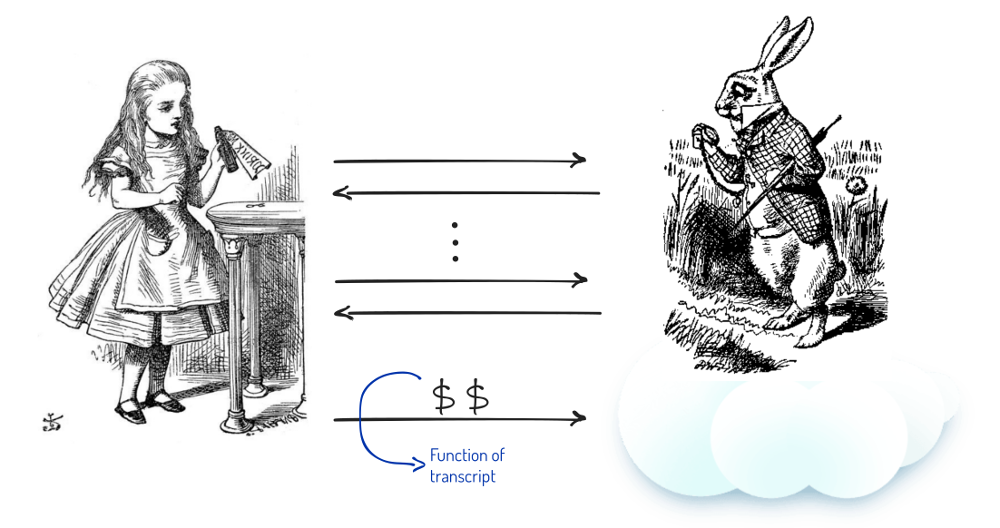
\includegraphics[scale=0.23]{pics/interaction.png}
\end{figure}
% Recall interactive proofs
% Recall our goal
\end{frame}


\begin{frame}{Rational Proofs: Definition [AM12]}
		\begin{framed}
			Let $f$ be a function and $(P,V)$ be a pair of algorithms. $(P,V)$ is a rational proof for $f$ if both:
			\onslide<+->
			\begin{enumerate}[<+- | alert@+>]
				\item \emph{("The honest prover always replies correctly")} 
				$$ \forall x\  \Pr[output(P,V)(x) = f(x) ] = 1$$
				\item \emph{("Any other prover will earn less than the honest one")}
				$$ \forall \disP \ \forall x \  \expRewProtHon - \expRewProtDis \geq \delta_{\disP}(x)  $$
				for some reward function $\rew$ and gap $\delta_{\disP}(x) \geq 0$
			\end{enumerate}
		\end{framed}
		
		%\pause
		%\vspace{0.5cm}
		%\center{\large{\textbf{What does $\rew$ look like?}}}
\end{frame}

\section{Rational Proofs for Feasible Computation}

\begin{frame}{Rational Proofs for Space-Bounded Computations}
\begin{block}{Theorem (informal)}
	If $L$ can be decided in time $T$ and space $S$ by a $DTM$, then it admits a rational proof with $O(\log n)$ rounds, $S \log n$ communication complexity and Verifier's running time.
\end{block}
\pause
\begin{itemize}[<+->]
	\item \textit{Special case:} If $T=poly(n)$ and $S=polylog(n)$ then we have a $O(\log n)$ round protocol with a polylog verifier.
	\item Generalization to randomized computation (using PRGs against space-bounded adversaries \cite{nisan1992pseudorandom}).
	\begin{itemize}
		\item unconditional PRGs
		\item Possible through one of our composition result.
	\end{itemize}
\end{itemize}
	% TODO: Say about generalization of result
\end{frame}

\begin{frame}{RPs for Space-Bounded Computations (intuition)}
\begin{itemize}
	\item Core: interactive proof with ``low'' soundness;\pause
	\item In the end, if verifier accepts, reward $R$ otherwise reward $0$
\end{itemize}
\medskip
\begin{figure}
	\pause
	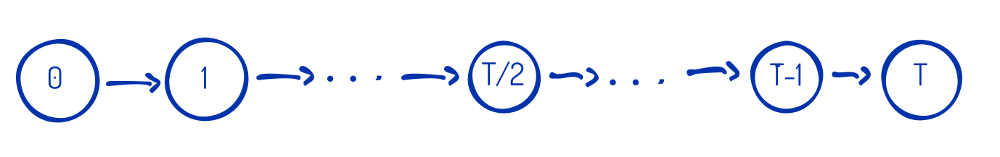
\includegraphics[scale=0.3]{pics/space-protocol.png}
	\caption{Configuration Graph of a deterministic computation}
\end{figure}
\end{frame}

\begin{frame}{How Efficient Can We Hope RPs for P to be?}
	\textbf{Our result for space-bounded (prev. slides):} For $S = \polylog(n)$ we have a polylog verifier and polylog total communication.
	\pause
	\begin{block}{Theorem (informal)}
It is unlikely\footnote{Unless ``something related'' to $\NP \subseteq \BPP$ holds} there exist rational proofs for P with polylog verification and log total communication;
\end{block}
\end{frame}


%
\section{On the Cost of Computation and Using Rational Proofs Multiple Times}

\begin{frame}{Computation has a Price: Accounting for Costs}
	\begin{columns}
	\column{0.60\textwidth}
	\begin{block}{So far:}
		\textit{Utility(worker)} $ = \function{Reward}$
	\end{block}
	\onslide<2->
	\begin{block}{Now :}
		\textit{Utility(worker)} $= \function{Reward} - \function{Cost}$
	\end{block}
	\column{0.40\textwidth}
	\onslide<3->
	\begin{block}{}
		$R - \tilde{R} \geq \delta \hspace*{\fill} (1) \hspace*{\fill}$
	\end{block}
	\onslide<4->
	\begin{block}{}
		$(R-C) - (\tilde{R}-\tilde{C}) \geq \delta \hspace*{\fill} (2) \hspace*{\fill}$			
	\end{block}
	\end{columns}
	\bigskip
		\onslide<5->
\begin{block}{How to achieve (2) given (1)?}
\end{block}
		\onslide<6->
	\begin{block}{Solution: scale reward appropriately}
		If (1) holds then scaling the reward function by a linear function of $C$ is sufficient to obtain (2).
	\end{block}
%[Say we can scale reward appropriately and this works for one-time]
% Say about individual rationality here
\end{frame}

\begin{frame}[t]{We May Still Have Issues with Multiple Proofs}
\large{\textbf{On input $x$:}}
\begin{columns}
	\column{0.5\textwidth}
\begin{block}{Honest prover $P$:}
	\begin{figure}
		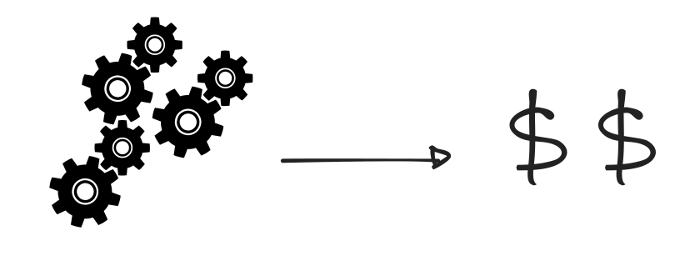
\includegraphics[scale=0.18]{pics/honest-rew.png}
	\end{figure}
\end{block}
\onslide<2->
	\column{0.5\textwidth}
%%%
\bigskip
\begin{block}{Some other prover $\disP$:}
	\begin{figure}
		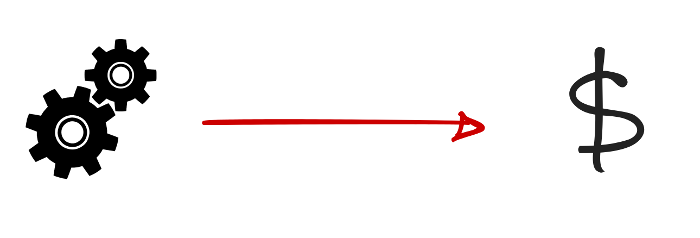
\includegraphics[scale=0.18]{pics/dishonest-rew-one.png}
	\end{figure}
\end{block}
\end{columns}
%%%
\onslide<3->
\large{\textbf{On multiple inputs $x_1, x_2, x_3$:}}
\begin{block}{The prover $\disP$ \underline{profits} more than $P$:}
	\begin{figure}
		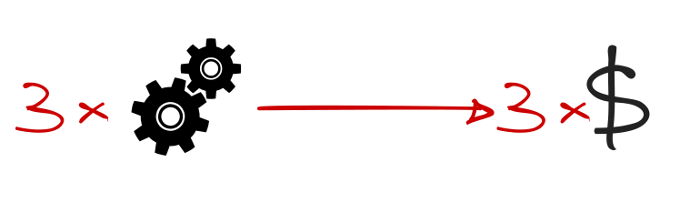
\includegraphics[scale=0.18]{pics/dishonest-rew-many.png}
	\end{figure}
\end{block}

\end{frame}

\begin{frame}[t]{Such Issue Do Occur in Rational Proofs}
	% TODO: Consider scaling between 0 and 1
	% Result: In Micali's protocol for threshold a random strategy is more profitable than an honest one
\large{\textbf{A worker can profit by just replying at random\footnote{A $O(1)$-cost strategy} in protocol by \cite{am1}.}}\onslide<2->
\medskip
\begin{columns}
	\column{0.60\textwidth}
	For a prover giving random answers:
	\onslide<2->
	\begin{align*}
	\tilde{R}_{rnd} > 1
	\end{align*}
	\onslide<3->
	Whereas for the honest prover:
	\[
	R^* \leq 2
	\]\\
	\medskip
	\onslide<4->
Therefore $2\tilde{R}_{rnd} > R^*$
{(It's more profitable to simply cheat twice)}
	\column{0.40\textwidth}
	\onslide<1->
	\begin{figure}
		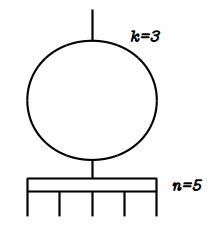
\includegraphics[scale=0.7]{pics/threshold-circ.png}
		
	\end{figure}
\end{columns}
\medskip
	\onslide<5-> \textbf{The protocol in \cite{am1} is not \textit{sequentially composable}}.
	\vfill
\end{frame}

\begin{frame}{Sequential Composability: A Definition}

\begin{framed}
\begin{block}{Desired Guarantee:}
	There should be little gain in doing several, \textit{incorrect} computations instead of a single correct one.
\end{block}
\end{framed}
	\bigskip
\pause
	\begin{block}{Definition}
		A rational proof $(P,V)$ for $f$ 
		is $\epsilon$-{\sf sequentially composable} for an input distribution $\cal D$, if:
			\pause
		\begin{itemize}
			\item  for every prover $\disP$, 
				\pause
			\item	$x,x_1,\ldots,x_k$ drawn according to ${\cal D}$,
		\end{itemize}
				\pause
		$$C(x) \geq \sum_{i=1}^k 
		\tilde{C}(x_i)\implies \sum_{i}\tilde{R}(x_i) - R \leq \epsilon$$
	\end{block}
\end{frame}

\begin{frame}{Sequential Composability: An Alternative Characterization}
\begin{figure}
	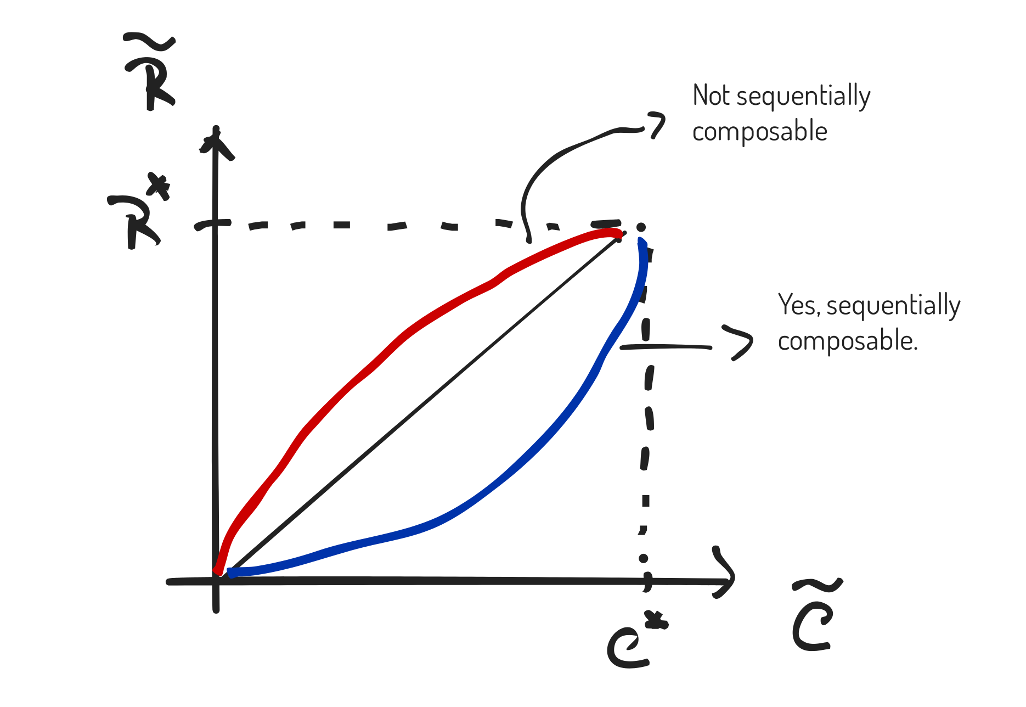
\includegraphics[scale=0.26]{pics/sc-char.png}
\end{figure}
$$ \tilde{C} > \tilde{R}$$
$$ \text{(assuming } R^* = C^* = 1)$$
\end{frame}

\begin{frame}{Space-Bounded Computation and Sequential Composability}
	% Mention cost assumption that we will talk about later
\begin{block}{Theorem (informal)}
	Our Rational Proof for Space Bounded Computation is Sequentially Composable.
\end{block}
\bigskip
\begin{figure}
	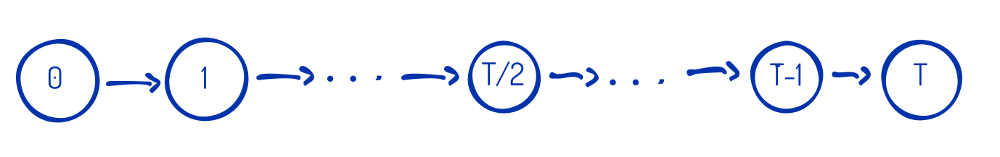
\includegraphics[scale=0.3]{pics/space-protocol.png}
%	\caption{Configuration Graph of a deterministic computation}
\end{figure}
\end{frame}

\begin{frame}[t]{Log-depth Arithmetic Circuits and Sequential Composability}
\begin{block}{Theorem (informal)}
There exist sequentially composable rational proofs for ``regular'' arithmetic circuits of $\log$-depth and $\poly$-size. with:
		\begin{itemize}
			\item $\log n$ rounds;
			\item polylog verifier.
			\item $O(T)$ prover.
		\end{itemize}
\end{block}

\begin{figure}
	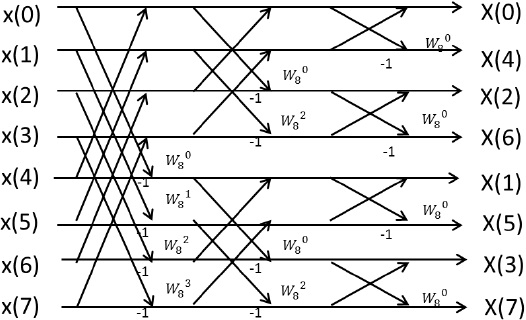
\includegraphics[scale=0.36]{pics/fft.jpg}
	\caption{Circuit for FFT}
\end{figure}
\end{frame}

\begin{frame}{Why Are These Protocols Sequentially Composable?}
	\begin{enumerate}
		\item Reward depends on ``checks'' (although with low soundness);\pause
		\begin{itemize}
			\item Different than other approaches where reward depends on \textit{scoring rules}.
		\end{itemize}\pause
		\item Assumptions on costs.
	\end{enumerate}
\end{frame}

\begin{frame}{On Cost Assumptions for Sequential Composability}
\begin{block}{Requirement (connecting cost and probability of guessing)}\pause
{\small 	It should not be too easy to guess a solution having done little work.} 
\end{block}	
	
\pause
\begin{figure}
	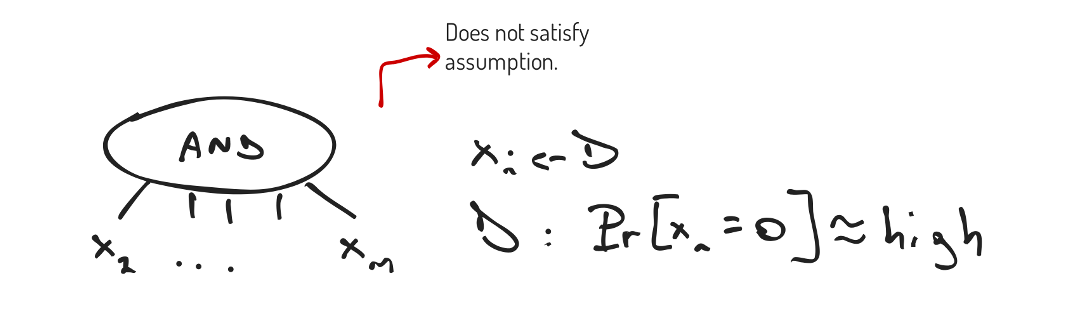
\includegraphics[scale=0.21]{pics/example-and.png}
\end{figure}
\pause
\begin{figure}
	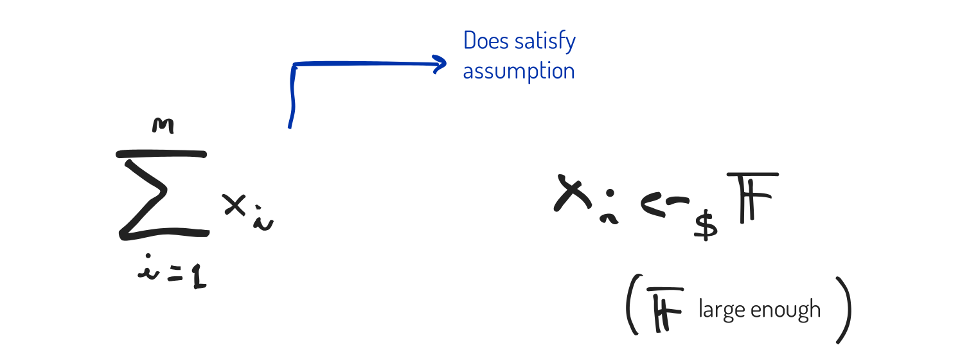
\includegraphics[scale=0.21]{pics/example-sum.png}
\end{figure}
\pause
\textbf{Our assumption:} guessing successfully w/ probability $p$ requires fraction of total work $p$.
\end{frame}

% == FG VC => Seq Comp ==
\section{Fine-Grained Protocols}

\begin{frame}{Two Perspectives on Fine-Grained Protocols}
	
	\begin{itemize}
		\item Cryptographic Perspective
		\item  Rational Perspective
	\end{itemize}
\end{frame}

\begin{frame}{Crypto Perspective}
	\textit{A FG protocol is one secure against a specific complexity class $\class{C}$}.\pause
	
	Examples in literature:
	\begin{itemize}
		\item Key-Exchange secure against $o(n^2)$ advs. (Merkle79)
		\item Maurer Space-Bounded
		\item DVV16
	\end{itemize}\pause
	Our result: A FG Verifiable Computation Protocol
\end{frame}

\begin{frame}{Rational Perspective}
\textit{In a FG protocol cheating costs strictly more than acting honestly.}\pause

\textbf{Theorem:} A FG Verifiable Computation scheme yields a sequentially composable rational proof.

[TODO: Image here with intuition/elaboration]
\end{frame}

% == Our main result: FG VC against NC1 adversaries from minimal assumptions ==
\begin{frame}{Our FG Verifiable Computation Scheme}
	[Result statement here]
\end{frame}

% == Additional properties ==
\begin{frame}{Properties of our VC scheme}
\end{frame}

% == How to obtain this VC: HE + transformation ==
% Say here that another result will be for HE
\begin{frame}{How to Obtain Fine-Grained VC}
	Core of our approach is \cite{ckv10}:
	\begin{itemize}
		\item  Obtains VC from Homomorphic Encryption (HE)
	\end{itemize}
\end{frame}

\def\E{\func{E}}

% == Homomorphic Encryption ==
\begin{frame}{Homomorphic Encryption (HE)}
	\begin{center} \textbf{HE = PKE + Evaluation Function} \end{center}
	\begin{enumerate}
		\item $\func{KeyGen} \to (\pk, \sk)$
		\item $\func{Enc}_{\pk}(x) \to \E(x)$
		\item $\func{Dec}_{\sk}(\E(x)) \to x$
		\pause  
		\item $\func{Eval}_{\pk}(f, \E(x)) \to \E(f(x))$
	\end{enumerate}
	\pause
	
	\begin{result}[HE against $\NC^1$ adversaries]
		TODO
	\end{result}
\end{frame}

% == VC from HE ==
\begin{frame}{VC from HE (\cite{ckv10})}
	TODO: Intuition of ckv10
	\begin{itemize}
		\item 
	\end{itemize}
	\pause
	\textbf{Enhancements:}
	\begin{itemize}
		% TODO: Improve graphics so that changes are clear
		\item \textbf{To amplify error:} use random permutation
		\item \textbf{To make reusable:} use HE  on top of construction.
	\end{itemize}
	% Scaling this up: error amplification (permutation); reusability
\end{frame}

% == VC from HE in low depth ==
\begin{frame}{Ensuring \cite{ckv10} works in low-depth}
	\textbf{Recall:} all our algorithms should run in $\NC^1$ and our verifier should be efficient.
	
	\textbf{Some of the issues to take care of: }
	\begin{itemize}
		\item Can we sample a random permutation in low-depth?
		\item We use ``double'' HE: $\function{Eval}(\function{Eval}(f, \cdot), c)$ stay in $\NC^1$?
%		\item How to make sure it works when HE has \textit{randomized} decryption? (our decryption is randomized, but the original construction only works for deterministic)
		\item In the proof, does the security reduction stay in $\NC^1$?
	\end{itemize}
\end{frame}

% == HE against NC1 circuits==
\begin{frame}{Obtaining our HE scheme}
	Our result: [TODO: restating our result]
	
	\textbf{Our approach:}
	\begin{enumerate}
		\item We start from the PKE secure against $\NC^1$ in \cite{fgcrypto};
		\item We apply relinearization techniques from \cite{fhe-lwe} to obtain HE;
		\begin{itemize}
			\item Can homomorphically evaluate polynomials of constant degree; 
		\end{itemize}
		\item We extend the class of functions we can evaluate homomorphically through degree reduction techniques from \cite{razborov1987lower}.
	\end{enumerate}\pause
	\textbf{Next, we see 1 and 2.}
\end{frame}

% == Description of DVV16 ==
\begin{frame}{PKE scheme from \cite{fgcrypto}}
	[TODO: Make more intuitive]
	\begin{itemize}
		\item $\PKEKeygen_{\sk}(\unlambda):$
		\begin{enumerate}
			\item Sample $(\M, \k) \gets \KSample(\unlambda)$;\\
			 {\color{red}(Property: if $\r$ random, $\transp{\r}  \M$ ``looks'' random to $\NC^1$ circuit)}
			\item Output $(\pk = \M, \sk = \k)$.
		\end{enumerate}
		\pause
		\item $\PKEEnc_{\pk}(\mu):$
		\begin{enumerate}
			\item Sample $\r \leftarrow_{\$} \bit^{\lambda}$;
			\item Let $\transp{t} = (0 \ \dots 0 \ 1) \in \bit^{\lambda}$;
			\item Output $\transp{\c} = \transp{\r}  \M + \mu\transp{\t}$.
		\end{enumerate}
		\pause
		\item $\PKEDec_{\sk}(\c):$
		\begin{enumerate}
			\item Output $\inprod{\k}{\c}$
		\end{enumerate}
		
	\end{itemize}
\end{frame}

\def\c{\vect{c}}
\def\cp{\vect{c'}}
\def\fc{f_{\c}}
\def\fcp{f_{\cp}}
\def\x{\vect{x}}

% == Description of relinearization ==
\begin{frame}{Relinearization step}
[TODO: Make all more intuitive]

 $  \fc(\x) = \inprod{\c}{\vect{x}} = \Sum c[i] x[i]$ \quad\quad\quad
 $  \fcp(\x) = \inprod{\cp}{\vect{x}} = \Sum c'[i] x[i]$
  \pause\\
 \medskip
 Homomorphic addition:
$$ \fc(\x)+\fcp(\x) = \inprod{\c+\cp}{\vect{x}}  = f_{\c+\cp}(\x) $$ 
\medskip 
\pause
Homomorphic multiplication:
 \begin{align*}
 \fc\cdot\fcp(\x)  & =   (\Sum c[i] x[i]) \cdot (\Sum c'[i]x[i]) \\
        				 & =  \Sum h_{i,j} x[i]x[j]   \quad\quad \small{( h_{i,j} \text{ obtained opening parenthesis})}
\end{align*}
\pause
\textbf{Problem:} now ciphertext this requires $\lambda^2$ bits.\pause

\textbf{Solution:} Provide $\vect{\rho}_{i,j} = \E(s[i]s[j])$ under a new secret key $\vect{t}$ as part of the public key.\pause
 
$
  \Sum h_{i,j} \vect{\rho}_{i,j}\pause  % TODO: Do bm
=  \Sum_{i,j,k} h_{i,j} \rho_{i,j}[k] t[k] \pause = \Sum_k t[k](\sum_{i,j} h_{i,j} \rho_{i,j}[k])\pause = f_{\c\cdot\cp}(\vect{t})
$
 
\end{frame}

\begin{frame}{Leveled Homomorphic Evaluation}
	[Intuition on doing relinearization at every level]
\end{frame} 

\section{Conclusions}

\begin{frame}{Summary}
		\begin{itemize}[<+- | alert@+>]	
			\item A critique of the model of rational proofs for multiple delegations;
			%\item A framework for multiple delegations (sequential composability);
			\item (Sequentially composable) protocols for $\log$-depth arithmetic circuits and space-bounded computations;
			\item VC and HE against $\NC^1$ adversaries and computable in low-depth;
			\begin{itemize}
				\item Under minimal assumptions.
			\end{itemize}
		\end{itemize}
\end{frame}

\begin{frame}{Related Work (Results on Rational Proofs)}
\begin{itemize}[<+- | alert@+>]
	\item First rational proof for space-bounded computation;
	\item $\cite{ratsumchecks}$ achieves constant-round \textit{rational arguments} for $\P$ (with cryptographic assumptions);
	\begin{itemize}
		\item Our results hold unconditionally;
	\end{itemize}
	\item \cite{rrr16} achieves constant-round interactive proofs for space-bounded computation;
	\begin{itemize}
		\item \cite{rrr16} has better round complexity;
		\item We fare better in terms of communication (us: polylog, \cite{rrr16}:$\poly(S(n)n^{\delta})$ and verification (us: sublinear, \cite{rrr16}: $\poly(S((n)) + n$).
	\end{itemize}
\end{itemize}
\end{frame}


\begin{frame}{Related Work (Results on Fine-Grained Protocols)}
	Comparison with information-theoretic results:
	\begin{itemize}[<+- | alert@+>]
		\item ``Proofs for Muggles'' \cite{muggles} obtains constant-round protocols for $\NC^1$.
		\begin{itemize}
			\item results in \cite{muggles} hold unconditionally; 
			\item our verifier runs in $\ACzt$; theirs in $\TC^0$;
			\item our protocol is I/O private and non-interactive.
		\end{itemize}
		\item \cite{gghkr07} obtains constant-depth ($\NC^0$) protocols for $\NC^1$.
		\begin{itemize}
			\item large verifier ($n^3$) and communication overhead.
		\end{itemize}
	\end{itemize}
\end{frame}

\begin{frame}{Future Work}
	\textbf{On Rational Proofs:}
	\begin{itemize}[<+- |  alert@+>]
		\item Rational proofs for $\P$ and $\NP$
		\item validating the model of rational proofs in the real world (How?)
		\item better parameters for the budget for rational proofs 
		% \item right now, the only parameter we use is n and we only require the budget to be poly(n). It'd be great to have a specific budget
		%		 parameter \beta, on the lines of the security parameter in crypto.
		%\item enforcing cost assumptions (with randomized encodings or other approaches)
		%		\item further applications of FG schemes to sequentially composable rational proofs
		%		 \item e.g. can one get a compiler from a stand alone rational scheme to a sequentially composable one having
	\end{itemize}
	\onslide<+->{
		\textbf{On Fine-Grained Crypto:}
		\begin{itemize}[<+- |  alert@+>]
			%\item pushing further on the partial results we have
			\item Other interesting crypto obtainable from $\L \neq \NC^1$ in a fine-grained model?
			\begin{itemize}
				\item Obfuscation? ABE? FE?
			\end{itemize}
			\item All the questions above, but with adversaries of \textit{bounded size} (instead of bounded depth)
			%\item FG primitives in the model of size as first step
		\end{itemize}
	}
\end{frame}

%
%\section{Rational Proofs for Space Bounded Computation}

\begin{frame}{One More Approach to Build Rational Proofs} % WIP
	\begin{itemize}[<+- | alert@+>]
		\item Scoring rules don't distinguish between different ``amounts of work''
		\item In fact, doing nothing gets you a fairly good reward (earlier example)
	\end{itemize}
	\onslide<+->
	\begin{block}{Another idea: ``Weak'' Interactive Proofs [BCEJKL08,AM13,CG15,CG17]}
		\begin{itemize}[<+- | alert@+>]
			\item Fix a reward $R^*$;
			\item Run an interactive protocol that returns \textsf{accept} or \textsf{reject}.
			\item Pay $R^*$ if it returns \textsf{accept}; $0$ otherwise.
		\end{itemize}
	\end{block}
	\onslide<+->
	We only need the \textit{test} to recognize a false answer with some ``not too small'' probability $\delta$.
	\onslide<+->
	
	\[
		 \expectation[\tilde{R}] \leq R^*(1-\delta)
	\]
	
\end{frame}

\begin{frame}{Rational Proofs for Bounded Space}
	\begin{block}{Theorem (informal)}
		If $L$ can be decided in time $T$ and space $S$ by a $DTM$, then it admits a rational proof with $O(\log T)$ rounds, $S \log T$ communication complexity and Verifier's running time.
	\end{block}
	\begin{itemize}[<+->]
		\item If $T=poly(n)$ and $S=polylog(n)$ then we have a $O(\log n)$ round protocol with a polylog verifier.		
	\end{itemize}
\end{frame}

\begin{frame}{Main Idea: Exploit the Configuration Graph}
	
	\begin{figure}
		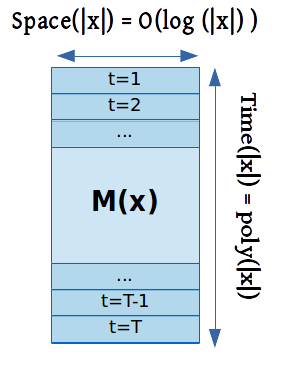
\includegraphics[scale=0.5]{pics/tm-rectangle.png}
	\end{figure}
	\begin{figure}
		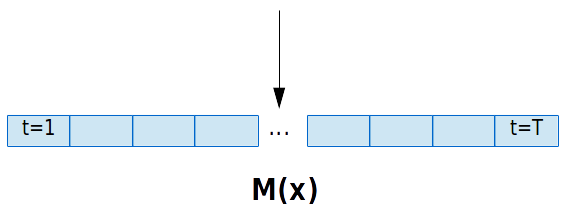
\includegraphics[scale=0.5]{pics/tm-lin.png}
	\end{figure}
\end{frame}

% r0
\begin{frame}{Execution Example}
	\begin{figure}
		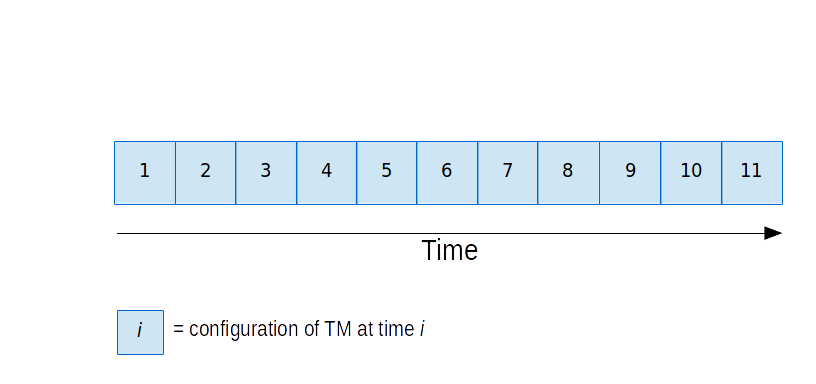
\includegraphics[scale=0.4]{pics/r0.png}
	\end{figure}
\end{frame}

%r1
\begin{frame}{Execution Example (cont.d)}
	\begin{itemize}
		\item $P$ sends $V$ the initial and final configurations .
	\end{itemize}
	\begin{figure}
		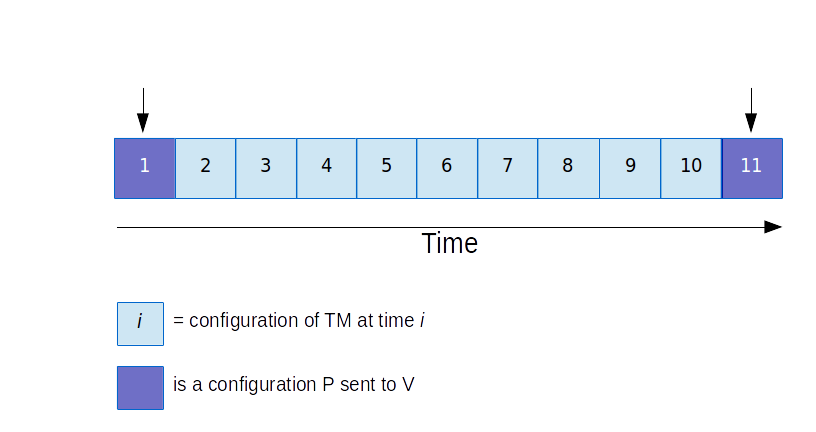
\includegraphics[scale=0.4]{pics/r1.png}
	\end{figure}
\end{frame}

%r2
\begin{frame}{Execution Example (cont.d)}
	
	\begin{itemize}
		\item $P$ sends $V$ the "midpoint" configuration (i.e. 6)
	\end{itemize}
	\begin{figure}
		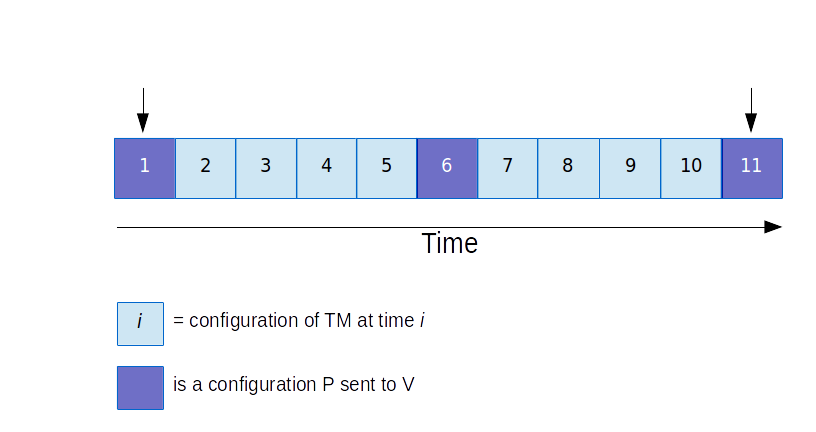
\includegraphics[scale=0.4]{pics/r2.png}
	\end{figure}
	
\end{frame}


%r2bis
\begin{frame}{Execution Example (cont.d)}
	\begin{itemize}
		\item $V$ flips a coin $b \in \{ 0,1 \}$. E.g. if $b = 0$, now the "window" of configurations shifts on the left half of the current window.
	\end{itemize}
	\begin{figure}
		
		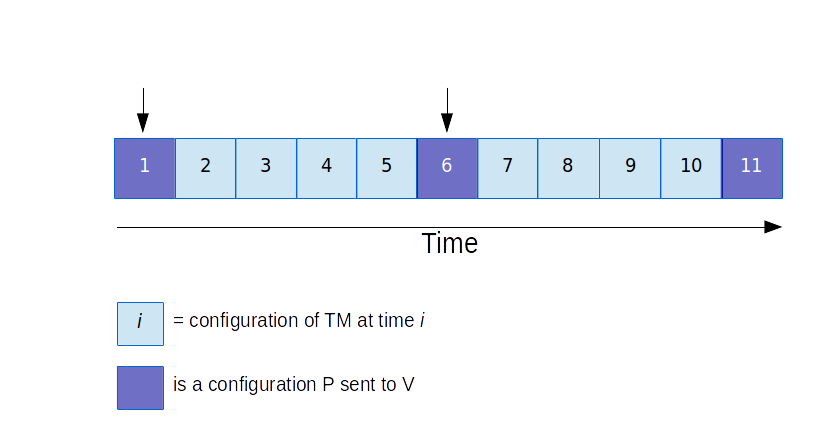
\includegraphics[scale=0.4]{pics/r2bis.png}
	\end{figure}
\end{frame}

%r3
\begin{frame}{Execution Example (cont.d)}
	\begin{itemize}
		\item $P$ sends $V$ the "midpoint" configurations (i.e. 3 and 4)
	\end{itemize}
	\begin{figure}
		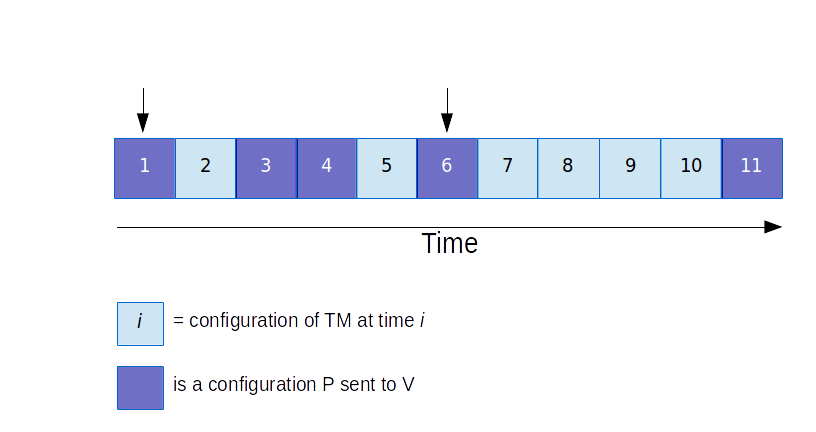
\includegraphics[scale=0.4]{pics/r3.png}
	\end{figure}
\end{frame}


%r3bis
\begin{frame}{Execution Example (cont.d)}
	\begin{itemize}
		\item $V$ flips a coin $b \in \{ 0,1 \}$. E.g. if $b = 1$, now the "window" of configurations shifts on the right half of the current window.
	\end{itemize}
	\begin{figure}
		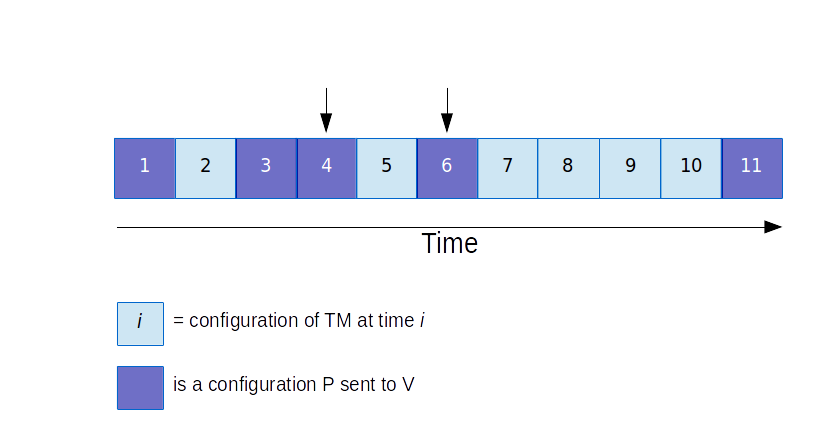
\includegraphics[scale=0.4]{pics/r3bis.png}
	\end{figure}
\end{frame}


%r-final
\begin{frame}{Execution Example (cont.d)}
	\begin{itemize}
		\item Now $V$ can check by itself that the transitions were consistent.
		\item $P$ receives reward $R$ only if final transition is consistent.
	\end{itemize}
	\begin{figure}
		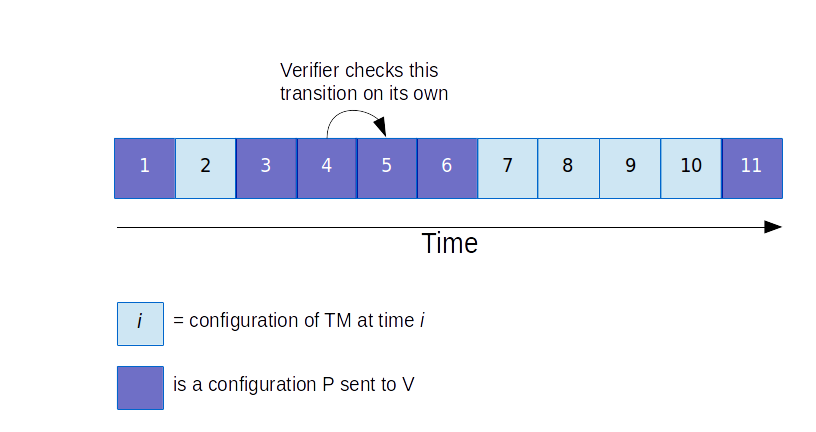
\includegraphics[scale=0.4]{pics/r-final.png}
	\end{figure}
\end{frame}


\begin{frame}{Analysis}
	\begin{block}{Efficiency}
	\begin{itemize}[<+- | alert@+>]
		\item The number of rounds is $O(\log T)$
		\item The Verifier's running time is $O(S \log T)$
	\end{itemize}
	\end{block}
	\onslide<+->
	\textbf{Rationality:} If the Prover cheats even on one transition it will lose in expectation a polynomial fraction of the honest reward.
	\onslide<+->
%	
%	\begin{block}{Sequential Composability (Intuition)}
%		\begin{itemize}[<+- | alert@+>]
%			\item If you haven't done all the work, then you are taking some risks in being found out;
%			\item The probability of being found out is proportional to the amount of work you haven't done;
%			\item Thus you'd be better off doing all the work.
%		\end{itemize}
%	\end{block}
%	\onslide<+->
%	\textbf{Caveat:} For that logic to work we need one more assumption.
\end{frame}

\begin{frame}{Sequential Composability (Intuition)}
		\begin{block}{Lemma (informal):}
			To achieve sequential composability it is sufficient to detect a cheating prover that invests $\tilde{C}$ with probability at least $\frac{\tilde{C}}{C^*}$

		\end{block}
	
		\onslide<+->
		\begin{block}{In the Last Protocol:}
		\begin{itemize}[<+- | alert@+>]
			\item If you haven't done all the work, then you are taking some risks in being found out;
			\item The probability of being found out is proportional to the amount of work you haven't done;
			\item Thus you'd be better off doing all the work.
		\end{itemize}
		\end{block}
	\onslide<+->
	\textbf{Caveat:} For that logic to work we need one more assumption.
\end{frame}

\begin{frame}{An Assumption on Cost}
		\begin{block}{}
		Investing at most a fraction $\gamma$ of the ``honest'' cost $\implies$ guessing $f(x)$ has probability at most\footnote<1->{plus some additive factor.} $\gamma$ 
	\end{block}
	
	\onslide<+->
	\begin{block}{Our results depend on this assumption. When does it hold?}
	\end{block}
	\onslide<+->
	\begin{itemize}[<+- | alert@+>]	
		\item It is unlikely interesting functions and distributions would satisfy \textit{directly} this assumption. (e.g. n-ary $\mathsf{AND}$).
		\item One option would be compiling $f$ into $\hat{f}$ where the assumption holds.
		\begin{itemize}
			\item possibly using approaches such as randomized encodings [IK00], proofs of useful work [BRSV17];
			\item \textbf{Left as future work.} (and not necessarily included in thesis).
			
		\end{itemize}
		\item \textbf{Next:} An alternative approach.
	\end{itemize}
	
\end{frame}
%
%

%
%\begin{frame}{This Talk}
	\begin{itemize}[<+- | alert@+>]	
	\item A critique of the model of rational proofs for multiple delegations;
	\item A framework for multiple delegations (sequential composability);
	\item Sequentially composable protocols for $\log$-depth arithmetic circuits and space-bounded computations.
	\item Verification schemes secure against $\NC^1$ adversaries. (in progress)
	\end{itemize}
\end{frame}
 % TODO: add open problems, comparison with related work

\begin{frame}{Additional Results}
\begin{itemize}[<+- | alert@+>]
	\item Lower Bounds for Rational Proofs for $\P$ and $\NP$
	\item Composition Theorem for Rational Proofs
	\item Rational Proofs for Randomized Computations
\end{itemize}
\end{frame}

\begin{frame}{Further Applications}
	\begin{itemize}[<+- | alert@+>]
		\item 	Cheap verification of smart contracts
		\begin{itemize}
			\item Something similar done in Ethereum (TrueBit).
		\end{itemize}
		\item Trusted computation with untrusted hardware components.
	\end{itemize}

\end{frame}


\begin{frame}{Rational Model vs Traditional Approaches}
	\begin{block}{What do we gain by assuming rationality?}
		\begin{itemize}[<+- | alert@+>]
			\item Efficiency
			\begin{itemize}
				\item Sublinear verification! (rational proofs)
				\item Low communication (also sublinear). (rational proofs)
			\end{itemize}
			\item Simplicity
			\item Minimal Assumptions
%			\begin{itemize}
%				\item These results hold even if OWFs do not exist
%				\item (\textit{Out of scope:} approaches using rationality+crypto )
%			\end{itemize}
		\end{itemize}
	\end{block}
	
%	\pause
%	% - The gains: efficiency, simplicity, lack of crypto
%	\begin{block}{Contrast with information-theoretic schemes:}
%		\begin{itemize}[<+- | alert@+>]
%			\item Comparable communication and worker's overhead (e.g [GKR08] vs [GHR16,\textbf{C}G15]; [RRR16] vs [\textbf{C}G17])
%			\item Verification is at least linear in information-theoretic setting.
%		\end{itemize}
%	\end{block}
\end{frame}




\begin{frame}{Open Problems}
	\textbf{On Rational Proofs:}
	\begin{itemize}[<+- |  alert@+>]
		\item Rational proofs for $\P$ and $\NP$
		\item validating the model of rational proofs in the real world (How?)
		\item better parameters for the budget for rational proofs 
		% \item right now, the only parameter we use is n and we only require the budget to be poly(n). It'd be great to have a specific budget
		%		 parameter \beta, on the lines of the security parameter in crypto.
		\item enforcing cost assumptions (with randomized encodings or other approaches)
		%		\item further applications of FG schemes to sequentially composable rational proofs
		%		 \item e.g. can one get a compiler from a stand alone rational scheme to a sequentially composable one having
	\end{itemize}
	\onslide<+->{
		\textbf{On crypto against limited adversaries:}
		\begin{itemize}[<+- |  alert@+>]
			%\item pushing further on the partial results we have
			\item Other interesting crypto obtainable from $\L \neq \NC^1$ in a fine-grained model?
			\begin{itemize}
				\item Obfuscation? ABE? FE?
			\end{itemize}
			\item All the questions above, but with adversaries of \textit{bounded size} (instead of bounded depth)
			%\item FG primitives in the model of size as first step
		\end{itemize}
	}
	
\end{frame}

\begin{frame}{}
	\Large Fin.
\end{frame}




\end{document}